\providecommand{\main}{..}
\documentclass[\main/notes.tex]{subfiles}

\begin{document}
	\ifSubfilesClassLoaded{\setcounter{chapter}{5}}{}
	\addtocontents{toc}{\protect\newpage}
	\chapter{Computer Networks and Internet}
		\section{Overview}
			\begin{definition}{Network}
				The interconnection of a set of devices capable of communication. A device can be:
				\begin{indentparagraph}
					\begin{description}
						\item[a host:] (or an \concept{end system}) -- the device that is at the end of the network
						\item[a connecting device:] a device that connects devices or networks.
							Examples are \concept{routers} (which connect networks), \concept{switches} (which connect devices), and \concept{modems} (which change the form of data.)
					\end{description}
				\end{indentparagraph}
				These devices are connected using wired or wireless transmission media.
			\end{definition}
			\begin{definition}{Local Area Network (LAN)}
				A privately owned network that connects hosts in a single office, building, or campus.

				Each host in a LAN has an address which is a unique identifier.
			\end{definition}
			\begin{definition}{Wide Area Network (WAN)}
				A network with a wider geographical span than a LAN. Interconnects connecting devices such as switches, routers, or modems. Normally created and run by communication companies, and leased by an organisation that uses it. Two distinct types:
				\begin{indentparagraph}
					\begin{description}
						\item[Point-to-point WAN] A network that connects two communicating devices through a transmission medium.
						\item[Switched WAN] A network with more than two ends. A combination of several point-to-point WANs, connected by switches.  
					\end{description}
				\end{indentparagraph}
			\end{definition}
			\begin{definition}{Internetwork (internet)}
				Two or more networks that are connected.
			\end{definition}

			\subsection{The Internet}
				\begin{definition}{The Internet}
					A network composed of thousands of interconnected networks.

					The top level of this are large backbone networks called \concept{international internet service providers (ISPs)}. These networks are connected through complex switching systems called \concept{peering points}.

					The second level contains smaller networks called \concept{provider networks}, or \concept{regional ISPs}.

					The third level contains \concept{customer networks} that actually use the services provided by the Internet.
				\end{definition}

			\subsection{Protocol Layering}
				\begin{definition}{Protocol}
					The rules that both the sender and receiver, and all intermediate devices, need to follow to be able to communicate effectively.
				\end{definition}
				\begin{definition}{Protocol Layering}
					Dividing a communication task into different layers, and defining a protocol for each layer.

					Some advantages are:
					\begin{indentparagraph}
						\begin{description}
							\item[Modularity] The layers are independent -- a layer (\concept{module}) can be replaced without needing to change everything. They can be thought of as a black box with inputs and outputs.
							\item[Separate services from implementation] A layer needs to receive a set of services, and send a set of services to the upper layer. The way it is implemented soes not need to be known.
							\item[Allows the use of intermediate systems] Systems don't have to use all the layers.
						\end{description}
					\end{indentparagraph}
				\end{definition}

				\subsubsection{Principles of Protocol Layering}
					\begin{enumerate}
						\item For bidirectional communication, each layer needs to perform two opposite tasks, one in each direction.
						\item The two objects under each layer at both sites should be identical -- they should be the same type.
					\end{enumerate}
				This means that there is a logical connecion at each layer.

			\subsection{TCP/IP Protocol Suite}
					\begin{definition}{TCP/IP (Transmission Control Protocol/Internet Protocol)}
						A \concept{protocol suite} (set of protocols organized in different layers) used in the Internet today. It is a \concept{hierarchical} protocol made up of interactive modules, each which provides a specific functionality.

						\begin{description}
							\item[Hierarchical] Each upper-level protocol is supported by services provided by one or more lower-level protocols.
						\end{description}
					\end{definition}

					There are $5$ layers:
					\newlist{LayerList}{enumerate}{1}
					\setlist[LayerList,1]{%
							label={\textbf{Layer \arabic*\addtocounter{LayerListi}{-2}}},
							align=left
					}
					\begin{indentparagraph}
						\begin{LayerList}[start=5]
							\item Application
							\item Transport
							\item Network
							\item Data Link
							\item Physical
						\end{LayerList}
					\end{indentparagraph}

					\begin{center}
						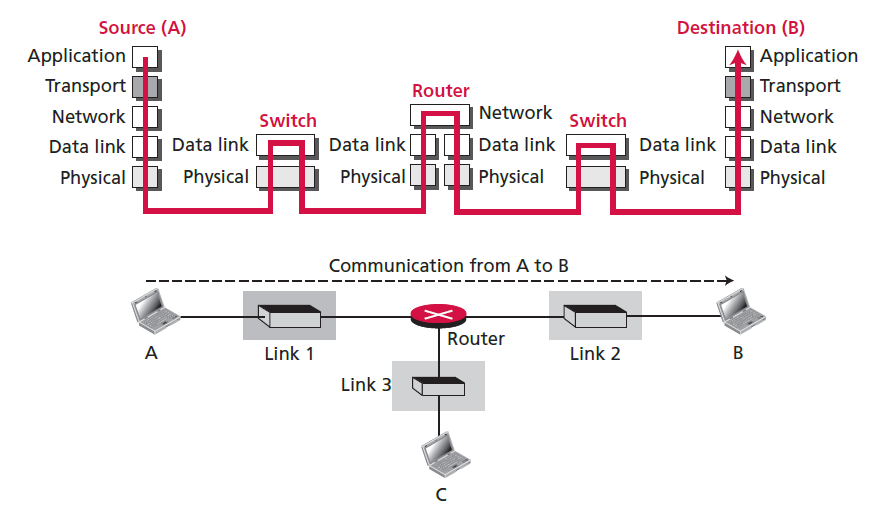
\includegraphics[width=0.9\textwidth]{\main/images/unit06/internet_layers.png}
					\end{center}
					Looking at the above image, each device is involved with a set of layers, but not necessarily all five. The two hosts (the source and destination) are involved with all $5$. The router is involved in only three, and the switches are involved in two.

					\pagebreak
					\subsubsection{Addressing and Packet Names}
						Each layer has a specific data type associated, as well as a specific type of address (except the physical layer, which cannot have an address).
						\begin{center}
							\begin{tabular}{ccc}
								Layer & Data & Address\\
								\midrule
								Application & Message & Names\\
								Transport & Segment/User Diagram & Port Numbers\\
								Network & Datagram & Logical Addresses\\
								Data Link & Frame & Link-layer addresses\\
								Physical & Bit & ---
							\end{tabular}
						\end{center}
						\begin{indentparagraph}
							\begin{description}
								\item[Application Layer] Names are used, such as \texttt{someorg.com} or \texttt{name@email.com}
								\item[Transport Layer] Port numbers are used. These define the application-layer programs at the source and the destination.

								A \concept{port number} is a local address that distinguishes between several running programs at the same time.
								\item[Network Layer] The addresses are global, with the whole Internet as the scope. Uniquely defines the connection of a device to the Internet.
								\item[Data-Link Layer] Locally defined addresses that define a specific host or router in a network. Also known as \concept{MAC addresses}.
							\end{description}
						\end{indentparagraph}

		\section{Application Layer}
			Provides services to the user. Does not provide services to any other protocol in the suite -- only receive services from the protocols in the transport layer.

			\subsection{Appplication Layer Paradigms}
				There are two possible paradigms for how application programs can communicate with each other: the \concept{client-server paradigm} and the \concept{peer-to-peer paradigm}.
				\begin{definition}{Client-Server Paradigm}
					The service provider is an application program, called the \concept{server process}. It runs continuously, waiting for another application program, called the \concept{client process}, to make a connection through the Internet. The role of each program is totally different --- they cannot operate as the other program.

					The server must be running the entire time; the client process is only run when the client needs to receive service. This means the concentration of the communication load is on the server, and therefore needs a powerful computer, which is expensive. This means the service should return some form of income.

					Examples are the \concept{World Wide Web (WWW)}, \concept{HyperText Transfer Protocol (HTTP)}, \concept{file transfer protocol (FTP)}, \concept{secure shell (SSH)}, and email.
				\end{definition}
				\begin{definition}{Peer-to-Peer Paradigm}
					Often abbreviated \concept{P2P paradigm}. No need for a server process to always run. The load is shared between peers: a computer can provide a service at one time, and receive a service at another, or at the same time.

					This paradigm is useful for \concept{Internet telephony} (calling via the Internet), or sharing files.

					Challenges related to this paradigm are security and applicability.
				\end{definition}

			\subsection{Standard Client-Server Applications}
				\subsubsection{World Wide Web and HTTP}
					\begin{definition}{World Wide Web}
						A repository of information in which the documents, called \concept{web pages}, are distributed all over the world, and related documents are linked together.

						Linking web pages is done using a concept called \concept{hypertext}, now also referred to as \concept{hypermedia}, as not just text can be linked this way.

						\begin{indentparagraph}
							\begin{description}
								\item[Hypertext] Using a machine that automatically retrieves another document stored in a system, when a link to the other document appears in the current document.
							\end{description}
						\end{indentparagraph}

						The WWW is a distributed client-server service, in which a client using a browser can access a service using a server. The service provided is distributed over many locations called \concept{sites}. Each site holds one or more documents, referred to as web pages. Each web page can contain links to other web pages in the same or different sites. They can therefore be either \concept{simple} or \concept{composite}.
						\begin{indentparagraph}
							\begin{description}
								\item[Simple Web Page] A webpage that has no links to other webpages
								\item[Composite Web Page] A webpage that has one or more links to other webpages.
							\end{description}
						\end{indentparagraph}

						Each webpage is a file with a unique name and address.
					\end{definition}
					\begin{definition}{Web Client (Browser)}
						Software that interprets and displays a weboage. Consists of three parts: a \concept{controller}, \concept{client protocols}, and \concept{interpreters}.
						\begin{indentparagraph}
							\begin{description}
								\item[Controller] Receives input from the keyboard or mouse, and uses the client programs to access the document. After the document has been accessed, the controller uses one of the interpreters to display the document on the screen.
								\item[Client Protocol] One of the protocols used to retrieve a document. Examples are \concept{HTTP} and \concept{FTP}.
								\item[Interpreter] Used to `translate' the document in a way that it can be displayed on screen. Depending on the type of document, this could be \concept{HTML (HyperText Markup Language)}, Java, or JavaScript. 
							\end{description}
						\end{indentparagraph}
					\end{definition}
					\begin{definition}{Web Server}
						The location where a web page is stored. Every time a request arrives, the corresponding document is sent to the client.
					\end{definition}
					\begin{definition}{Uniform Resource Locator (URL)}
						A unique identifier for a web page, that distinguishes it from other web pages. Requires three identifiers to be defined: \concept{host}, \concept{port}, and \concept{path}. The browser also needs to know what client-server application to use -- the \concept{protocol}.
						\begin{indentparagraph}
							\begin{description}
								\item[Protocol] An abbreviation for the client-server program that we need in order to access the webpage.
								\item[Host Identifier] IP address or unique name given to a server
								\item[Port] A $16$-bit integer, usually predefined for the client-server application
								\item[Path] The location and name of the file in the underlying operating system. The format of this depends on the operating system.
							\end{description}
							\begin{center}
								\texttt{protocol://host/path}\\
								\texttt{protocol://host:port/path}
							\end{center}
						\end{indentparagraph}
					\end{definition}
					\begin{definition}{HyperText Transfer Protocol (HTTP)}
						A protocol used to define how the client-server programs can be written to retrieve webpages from the Web.

						An HTTP client sends a request, an HTTP server returns a response. The server uses the port number $80$, the client uses a temporary port number.
					\end{definition}
				\pagebreak
				\subsubsection{File Transfer Protocol (FTP)}
					\begin{definition}{File Transfer Protocol (FTP)}
						The standard protocol provided by TCP/IP for copying a file from one host to another.

						The client has three components: \concept{user interface}, the \concept{client control process}, and the \concept{client data transfer process}.

						The server has two components: the \concept{server control process}, and the \concept{server data transfer process}.

						The \concept{control connection} is made between the control processes. The \concept{data connection} is made between the data transfer processes.

						\begin{center}
							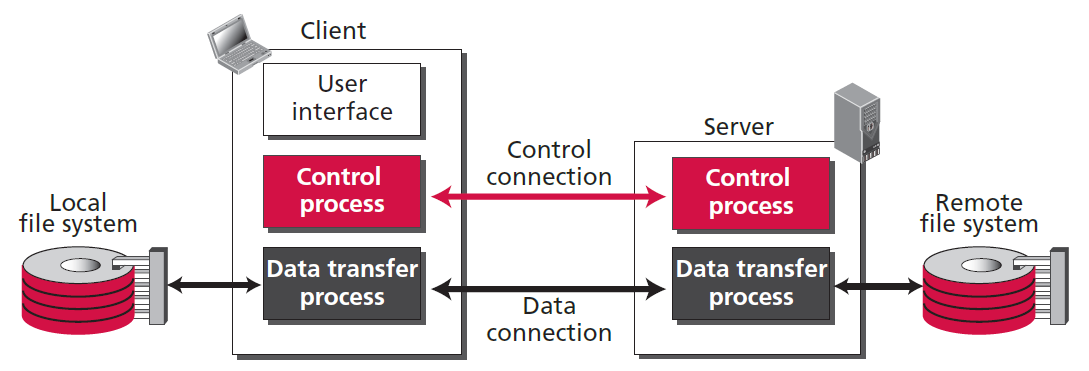
\includegraphics[width=0.9\textwidth]{\main/images/unit06/ftp.png}
						\end{center}

						The control connection remains connected during the entire interactive FTP session. The data connection is opened and then closed for each file transfer activity.
					\end{definition}
				\subsubsection{Electronic Mail (Email)}
					\begin{definition}{Electronic Mail (Email)}
						Allows users to exchange messages. Unlike the other applications, this is considered a \concept{one-way transaction}. Also, the receiver and sender of the mail does not run a server program. Therefore, intermediate computers (servers) should be used.

						Sender and receiver are connected via LAN or WAN to two mail servers. On the server, a mailbox is created for each user, where the received messages are stored. A queue (\concept{spool}) is created to store messages waiting to be sent.
						\begin{indentparagraph}
							\begin{description}
								\item[Mailbox] Part of a server hard drive, a special file with permission restrictions. Only the owner of the mailbox has access to it.
							\end{description}
						\end{indentparagraph}
						\begin{center}
							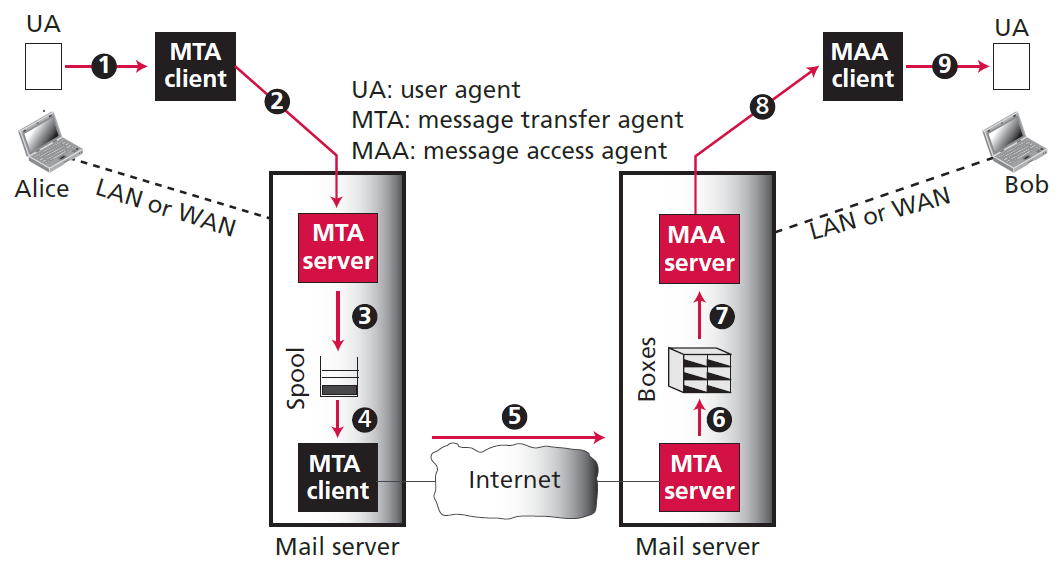
\includegraphics[width=0.9\textwidth]{\main/images/unit06/email.png}
						\end{center}
						A simple email takes nine different steps, and uses three different \concept{agents}: a \concept{user agent (UA)}, a \concept{Mail Transfer Agent (MTA)}, and a \concept{Message Access Agent (MAA)}.
						\begin{enumerate}
							\item Sender runs a UA program to prepare the message and send it to the mail server
							\item The UA triggers the MTA client which sends the message to the mail server
							\item The mail server uses a spool to store messages waiting to be sent
							\item From the spool, the MTA client is triggered, as there is a message in the queue
							\item The MTA client sends the message via the Internet
							\item The MTA server, which is always running, receives the message
							\item The message is stored in a mailbox on the server
							\item In order to access the messages in the mailbox, an MAA client is used
							\item The receiver runs a UA program to access messages from the mail server, which is connected to the MAA client
						\end{enumerate}
					\end{definition}
				\subsubsection{TELNET (Terminal Network)}
					\begin{definition}{Remote Login}
						A generic client/server program that allows a user on the client site to log into the computer on the server site and use the services available there.
					\end{definition}
					\begin{definition}{TELNET (TErminaL NETwork)}
						An original remote logging protocol. Requires a logging name and password, but is vulnerable to attack, as all data is sent in \concept{plaintext}. Due to this, the use of this has diminished in favour of \concept{Secure Shell (SSH)}.
					\end{definition}
				\subsubsection{Secure Shell (SSH)}
					\begin{definition}{Secure Shell}
						A secure application program that can be used for several purposes including remote logging, and file transfer. Originally designed to replace TELNET.

						Two versions, which are incompatible with each other, exist: SSH-1 and SSH-2. SSH-1 has been deprecated due to security flaws.
					\end{definition}
				\subsubsection{Domain Name System (DNS)}
					\begin{definition}{Domain Name System (DNS)}
						A directory system that maps a name to an IP address. This is distributed among many computers. The host that needs mapping can contact the closest computer holding the required information.
						\begin{enumerate}
							\item User passes the host name to the file transfer client.
							\item File transfer client passes the host name to the DNS client.
							\item Each computer knows the address of one DNS server. The DNS client sends a message to the DNS server with a query that gives the file transfer server name using the known IP address of the DNS server.
							\item DNS server responds with the IP address of the desired file transfer server.
							\item DNS client passes the IP address to the file transfer server.
							\item File transfer client now uses the received IP address to access the file transfer server.
						\end{enumerate}
						\begin{center}
							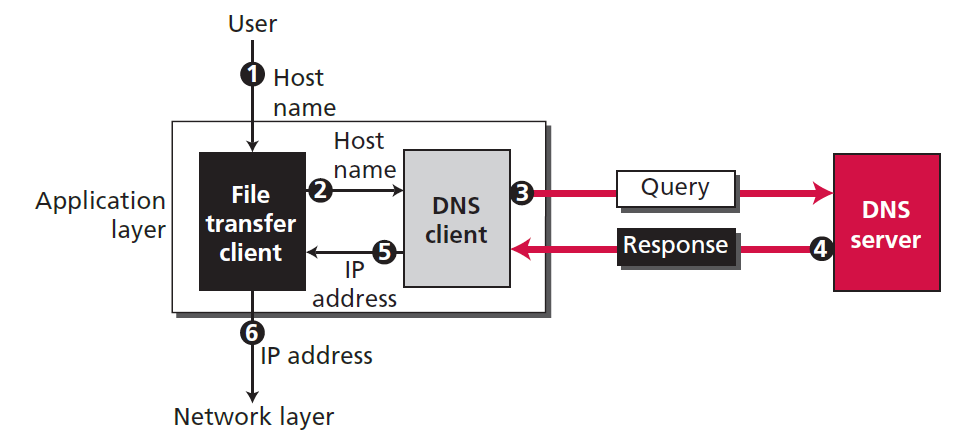
\includegraphics[width=0.9\textwidth]{\main/images/unit06/dns.png}
						\end{center}
					\end{definition}
					For DNS, the names assigned to machines must be unique. A \concept{name space} can map each address to a unique name. These are normally organized hierarchically.

					\pagebreak
					\paragraph{DNS in the Internet} The \concept{domain name space} was originally devided into three different sections: \concept{generic domains}, \concept{country domains}, and \concept{inverse domains}. Inverse domains are now deprecated.
					\begin{indentparagraph}
						\begin{description}
							\item[Generic Domains] Registered hosts according to their generic behaviour.
								\begin{center}
									\begin{tabular}{llll}
										Label & Description & Label & Description\\
										\midrule
										\texttt{.aero} & Airplanes and Aerospace       & \texttt{.int}    & International Organisations\\
										\texttt{.biz}  & Businesses or Firms           & \texttt{.mil}    & Military Groups\\
										\texttt{.com}  & Commercial Organisations      & \texttt{.museum} & Museums\\
										\texttt{.coop} & Cooperative Organisations     & \texttt{.name}   & Personal Names\\
										\texttt{.edu}  & Educational Institutions      & \texttt{.net}    & Network Support Centres\\
										\texttt{.gov}  & Governmental Institutions     & \texttt{.org}    & Nonprofit Organisations\\
										\texttt{.info} & Information Service Providers & \texttt{.pro}    & Professional Organisations
									\end{tabular}
								\end{center}
							\item[Country Domains] Use two-character country abbreviations. Second labels can be more specific, national locations, or organisational.
						\end{description}
					\end{indentparagraph}

			\subsection{Peer-to-Peer Applications}
				The first instance of P2P file sharing was December 1987, when Wayne Bell created \concept{WWIVNet}, the network component of WWIV (World War Four) bulletin board software.

				In July 1999, Ian Clarke designed \concept{Freenet}, a decentralised, censorship-resistant distributed data store.

				P2P gained popularity through \concept{Napster}, an online music file sharing service created by Shawn Fanning.

				P2P networks can be divided into two categories: \concept{centralised networks}, and \concept{decentralised networks}.
				\subsubsection{Centralised Networks}
					\begin{definition}{Centralised Network}
						The directory system listing of the peers and what the offer uses the client-server paradigm, but the storing and downloading of the files are done using the P2P paradigm. Sometimes referred to as a \concept{hybrid P2P network}.

						The peer first registers itself with a central server. The peer then provides its IP address, and a list of files it has to share.

						A peer, looking for a particular file, sends a query to the central server. The server searches its directory, and responds with the IP addresses of nodes that have a copy of the file.

						\begin{indentparagraph}
							\begin{description}
								\item[Advantages] Maintenance of the directory is simple.
								\item[Disadvantages] Accessing the directory can generate huge traffic, and slow down the system. The central servers are vulnerable to attack.
							\end{description}
						\end{indentparagraph}
					\end{definition}
				\subsubsection{Decentralised Networks}
					\begin{definition}{Decentralised Network}
						Does not depend on a centralised directory system. Instead, peers arrange themselves into an \concept{overlay network}.
						\begin{indentparagraph}
							\begin{description}
								\item[Overlay Network] A logical network made on top of the physical network.
							\end{description}
						\end{indentparagraph}
						Depending on the way the nodes in the overlay network are linked, a decentralised P2P network can be either \concept{unstructured} or \concept{structured.}
						\begin{indentparagraph}
							\begin{description}
								\item[Unstructured] Nodes are linked randomly. A search is not very efficient, because a query for a file must be flooded through the network, which produces significant traffic, and the query may still not be resolved. Examples are \concept{Gnutella} and \concept{Freenet}.
								\item[Structured] Uses a predefined set of rules to link nodes, so that a query can be effectively and efficiently resolved. The most commot technique is the \concept{Distributed Hash Table (DHT)}. DHT is used in many applications, such as \concept{Distributed Data Structure (DDS)}, \concept{Content Distributed Systems (CDS)}, \concept{Domain Name System (DNS)}, and P2P.
							\end{description}
						\end{indentparagraph}
					\end{definition}

		\section{Transport Layer}	
			Located between the application layer and the network layer. Provides services to the application later, and receives services from the network layer.

			Acts as a liaison between a client program and a server program.
			\subsection{Transport Layer Services}
				\subsubsection{Process-to-Process Communication}
					\begin{definition}{Process-to-Process Communication}
						This is the first duty of a transport-layer protocol. Responsible for deliver of the message to the appropriate process.
							\begin{indentparagraph}
								\begin{description}
									\item[Process] An application-layer entity that uses the services of the transport layer.
								\end{description}
							\end{indentparagraph}
					\end{definition}
					\begin{definition}{Addressing: Port Numbers}
						Most common way to achieve process-to-process communication is through the client-server paradigm.

						For communication, the local host, local process, remote host, and remote process must all be defined. The hosts are defined using IP addresses. The processes require a second identifier, called a \concept{port number}. Port numbers are $16$-bit integers from $0$ to $65536$.

						The client program defines itself with a port number, called the \concept{ephemeral port number}, meaning \emph{short-lived}. Recommended to be greater than $1023$. This number is temporary.

						The server also defines itself with a port number. This is not chosen randomly -- TCP/IP uses universal port numbers for servers, called \concept{well-known port numbers}. This number is permanent.
					\end{definition}
			\subsection{Transport Layer Protocols}
				Many different protocols, two are discussed: \concept{UDP} and \concept{TCP}.
				\subsubsection{User Datagram Protocol (UDP)}
					\begin{definition}{User Datagram Protocol (UDP)}
						A connectionless, unreliable transoprt protocol. Does not add anything to the services of the network layer, except providing process-to-process communication instead of host-to-host communication.

						Very simple proyocol using a mininum of overhead. If a process wants to send a small message, and does not care about reliability, UDP can be used.

						Much less interaction between the sender and receiver than using TCP.
					\end{definition}
					\begin{definition}{User Datagrams}
						UDP packets, that have a fixed-size \concept{header} of $8$ bytes. This is stored in an \concept{IP datagram} with a total length of $65\,535$ bytes.
						\begin{center}
							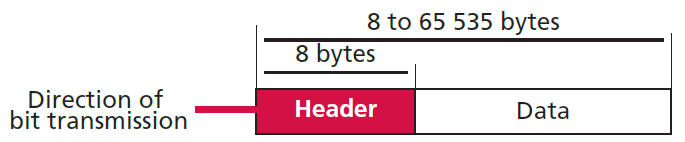
\includegraphics[width=0.5\textwidth]{\main/images/unit06/user_datagram.png}
						\end{center}
					\end{definition}
				\subsubsection{Transmission Control Protocol (TCP)}
					\begin{definition}{Transmission Control Protocol (TCP)}
						A connection-oriented, reliable transport protocol. Explicitly defines connection establishment, data transfer, and connection teradown phases, to provide a connection-oriented service.
						\begin{indentparagraph}
							\begin{description}
								\item[Connection-oriented service] There is a connection/relationship between all packets (\concept{segments}) belonging to the same message.
							\end{description}
						\end{indentparagraph}
						Uses sequence numbers to define the order of the segments. The sequence number is related to the number of bytes in each segment. In this way, if a sequence is list, the receiver holds the other sequences until the lost one is resent by the sender.
					\end{definition}
					\begin{definition}{Segments}
						A TCP packet -- a group of bytes. TCP adds a header to each segment (for control purposes) and delivers the segment to the network layer for transmission. The segments are encapsulated in an IP datagram.
						\begin{center}
							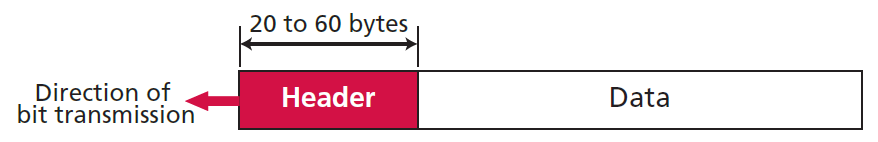
\includegraphics[width=0.6\textwidth]{\main/images/unit06/tcp_segments.png}
						\end{center}
					\end{definition}

		\section{Network Layer}
			Responsible for the host-to-host delivery of messages. Involved at the source host, destination host, and all routers in the path.

			At the source host, the network layer accepts a packet from the transport layer, encapsulates the packet in a \concept{datagram}, and delivers the packet to the data-link layer.

			At the destination host, the datagram is decapsulated, the packet is extracted and delivered to the corresponding transport layer.

			Routers use three layers if they are only routing packets -- they may use the transport and application layers for control purposes. Routers are normally shown with two data-link layers, and two physical layers, because they receive a packet from one network, and deliver it to another network.

			\subsection{Network Layer Services}
				\subsubsection{Packetizing}
					\begin{definition}{Packetizing}
						Encapsulating the payload in a network-layer packet at the source, and decapsulating the payload from the network-layer packet at the destination.
						\begin{indentparagraph}
							\begin{description}
								\item[Payload] Data received from the upper layer.
							\end{description}
						\end{indentparagraph}
						Done in three steps:
						\begin{enumerate}
							\item The source network-layer protocol receives a packet from the transport-layer protocol, adds a header that contains the source and destination addresses, and some other information that is required by the network-layer protocol.
							\item The network layer protocol then logically delivers the packet to the network-layer protocol at the destination.
							\item The destination host receives the network-layer packet, decapsulates the payload, and delivers the packet to the upper-layer protocol.
						\end{enumerate}
						\begin{center}
							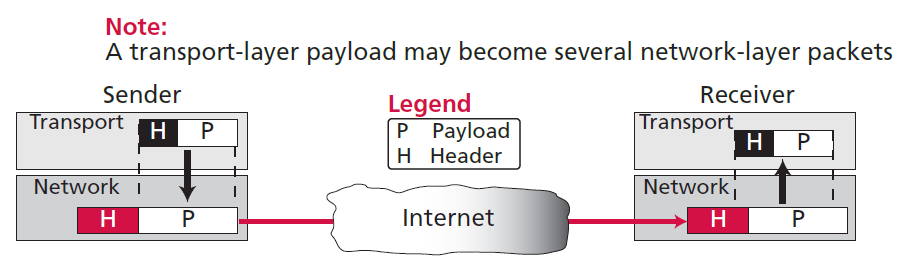
\includegraphics[width=0.9\textwidth]{\main/images/unit06/network_packets.png}
						\end{center}
						If the packet is fragmented at the source or at the routers, the network layer is responsible for waiting until all fragments arrive, reassembling them, and delivering them to the upper layer protocol.
					\end{definition}
				\pagebreak
				\subsubsection{Packet Delivery}
					Packet delivery at the network layer is \concept{unreliable} and \concept{connectionless}.
					\begin{definition}{Unreliable Delivery}
						Packets can be corrupted, lost, or duplicated. The network layer provides a best-effort delivery, but there is no guarantee that a packet will reach the destination.

						If a guarantee is needed, the delivery of packets would be delayed, as each packet would need to be checked at each router and destination, and resent if correupted. Checking for lost packets is even more costly.

						Therefore, to properly guarantee the messages are not corrupted, use the TCP protocol at the transport layer. If a payload at the transport layer is corrupted or lost, TCP drops the packet and requests resending of the data.
					\end{definition}
					\begin{definition}{Connectionless Delivery}
						The network layer treats each packet independently -- there is no relationship between packets belonging to the same transport-layer payload. There is no guarantee that the packets will arrive in the same order they were sent, as each packet may follow a different path.
						\begin{center}
							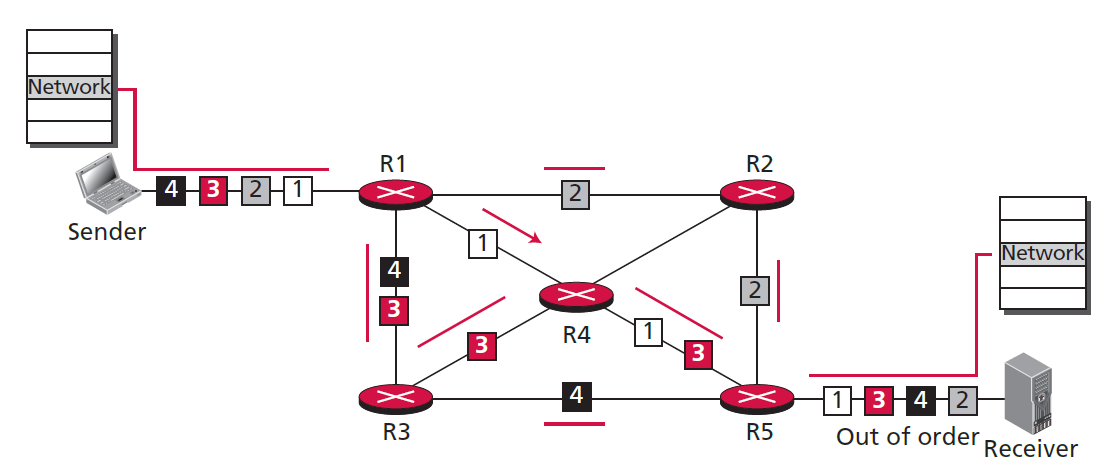
\includegraphics[width=0.9\textwidth]{\main/images/unit06/packet_paths.png}
						\end{center}
						The transport layer at the destination is responsible for holding packets until all of them arrive, before putting them in order, and delivering them to the application layer.
					\end{definition}
				\subsubsection{Routing}
					\begin{definition}{Routing}
						Route the packet from the source to the destination. A physical network is a combination of networks, which means there are multiple routes from the source to the destination. The network layer is responsible for determining which route is the best amont the routes. There are \concept{routing protocols} that are used to help find the best route.
					\end{definition}
			\subsection{Network Layer Protocols}
				While there are several protocols at this layer, the main one is \concept{Internet Protocol (IP)}. There are two versions: \concept{IPv4} and \concept{IPv6}.
				\subsubsection{Internet Protocol Version 4 (IPv4)}
					Most sytems use this protocol, but this will be changed in future, due to a smaller address space and packet format.
					\begin{definition}{IPv4 Addressing}
						Used to identify the connection of each device to the Internet. This is a $32$-but address that uniquely and universally defines the connection of a host or a router to the Internet.

						The IP address is the address of the \emph{connection}, not the host or the router. If a device is moved to another network, the IP address mat be changed.

						Unique in the sense that each address defines one, and \emph{only} one, connection to the Internet.

						There are three common notations to show an IPv4 address: \concept{binary notation} (base $2$), \concept{dotted-decimal notation} (base $256$), and \concept{hexadecimal notation} (base $16$).
						\begin{indentparagraph}
							\begin{description}
								\item[Binary Notation] Displayed as $32$ bits. One or more spaces is usually inserted between each byte.
								\item[Dotted-Decimal Notation] Each byte is converted to decimal, and is separated by a dot. Each number is between $0$ and $255$.
								\item[Hexadecimal Notation] Each hexadecimal digit is equivalent to $4$ bits. A $32$-bit address has $8$ hexadecimal digits. Often used in network programming.
							\end{description}
						\end{indentparagraph}
						\begin{example}
							Different forms of the same IP address:
							\begin{indentparagraph}
								\begin{description}
									\item[Binary] $10000001\;00000011\;00000111\;00011110$
									\item[Dotted-Decimal] $ 129.3.7.30$
									\item[Hexadecimal] $8103071$E
								\end{description}
							\end{indentparagraph}
						\end{example}
						This address is hierarchical, and divided into two parts. The first part of the address, called the \concept{prefix}, defines the network. The second part of the address, called the \concept{suffix}, defines the node. The prefix and suffix lengths depend on the size of the network. If the prefix length is $n$ bits, the suffix length is $(32 - n)$ bits.
					\end{definition}
					\pagebreak
					\begin{definition}{IPv4 Datagram}
						Packets used by IP are called \concept{datagrams}. A \concept{datagram} is a variable-length packet consisting of two parts: a \concept{header} and \concept{payload} The header is $20$ to $60$ bytes in length, and contains information essential to routing and delivery.
						\begin{center}
							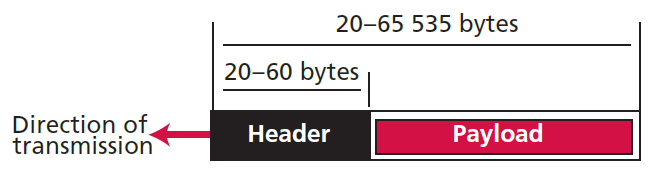
\includegraphics[width=0.6\textwidth]{\main/images/unit06/ipv4_datagram.png}
						\end{center}
					\end{definition}
				\subsubsection{Internet Protocol Version 6 (IPv6)}
					Shortcomings of IPv4, such as address depletion, led to the development of a new IP protocol. \concept{IPv6}, also called \concept{IP new generation (IPng)} augments trhe address space of IPv4, and redesigns the format of the IP packet.
					\begin{definition}{IPv6 Addressing}
						To prevent address depletion, IPv6 uses $128$ bits to define any device connected to the Internet. This address is represented as either \concept{binary}, or \concept{colon-hexadecimal form}. The first form is used to store an address in the computer, the second form is used by humans.
						\begin{example}
							Forms of IPv6 addresses:
							\begin{indentparagraph}
								\begin{description}[nosep]
									\item[Binary] $1111111011110111 \cdots 0001001101000101$
									\item[Colon-Hexadecimal] FEF7:5623:0017:A2B5:BC21:0243:7256:1345
								\end{description}
							\end{indentparagraph}
						\end{example}
						Defines three levels of hierarchy: site, subnetwork, and connection to the host.
						\begin{center}
							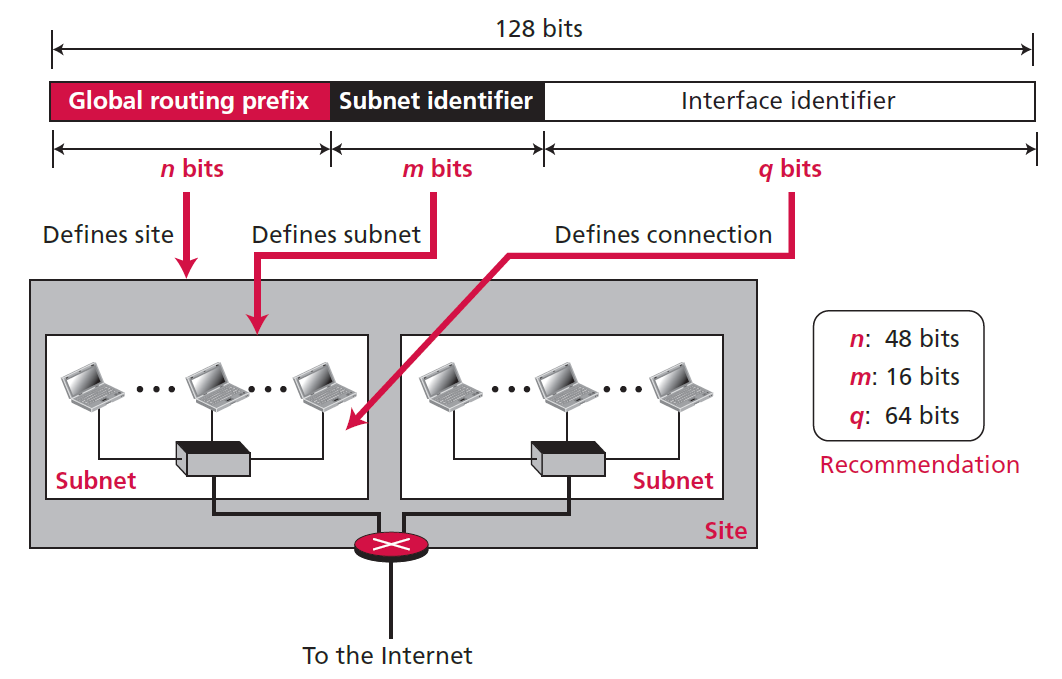
\includegraphics[width=0.8\textwidth]{\main/images/unit06/ipv6_address.png}
						\end{center}
					\end{definition}
					\begin{definition}{IPv6 Datagram}
						Also a variable length packet consisting of two parts: header and payload. The header is $40$ bytes. However, some extension headers are considered part of the payload in this version.
						\begin{center}
							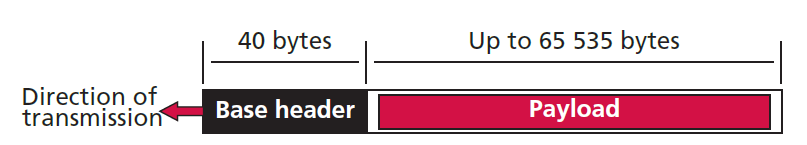
\includegraphics[width=0.6\textwidth]{\main/images/unit06/ipv6_datagram.png}
						\end{center}
					\end{definition}

		\section{Data-Link Layer}
			TCP/IP does not define any protocol in this layer. This is the territory of networks that, when connected, make up the Internet. There are several standard protocols in the market today.
			\subsection{Nodes and Links}
				While communication at the upper layers is end-to-end, at the data-link layer communication is \concept{node-to-node}.
				Data units from one point in the Internet need to pass through many networks to reach another point. These networks are connected by routers. The two hosts, and each router, is referred to as a \concept{node}, and the networks in between are referred to as \concept{links}.
				The links that connect the nodes are either \concept{local area networks (LANs)} or \concept{Wide Area Networks (WANs)}.
			\subsection{Local Area Networks (LANs)}
				LANs can be either \concept{wired} -- connected by wire, or \concept{wireless} -- connected by air.
				\subsubsection{Wired LANs}
					\begin{definition}{Ethernet}
						Developed in the 1970s by Robert Metcalfe and David Boggs. Has gone through four generations. The \concept{data rate} (the speed in which bits are sent in each second) has increased ten times in each generation.
						\begin{indentparagraph}
							\begin{description}
								\item[Standard Ethernet (10 Mbps)] A group of bits are packaged together in a \concept{frame} and sent together. The fram also carries information such as the \concept{source address} ($48$ bits), the \concept{destination address} ($48$ bits), the type of data, the actual data, and some other control bits to help check data integrity.
									\begin{center}
										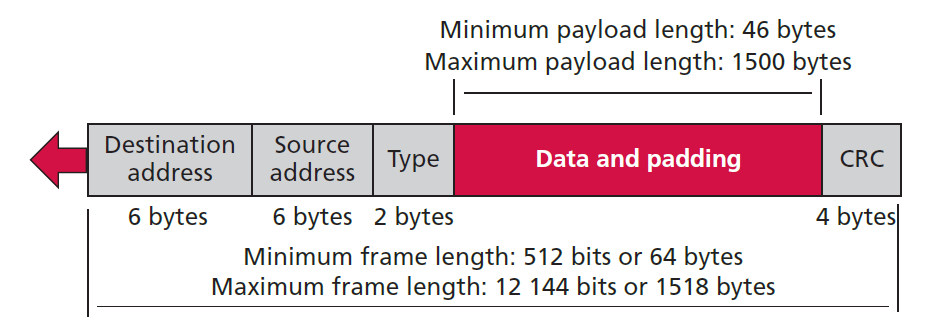
\includegraphics[width=0.7\textwidth]{\main/images/unit06/ethernet_frame.png}
									\end{center}
								\pagebreak
								\item[Fast Ethernet (100 Mbps)] The \concept{transmission rate} (or data rate) is increased, but is still compatible with Standard Ethernet.
								\item[Gigabit Ethernet (1000 Mbps)] Upgrades the data rate, but keeps the address length, frame format, and the maximum and mininum frame length the same.
								\item[10-Gigabit Ethernet] Extend the technology, data rate, and coverage distance so Ethernet can be used as LAN and \concept{MAN (metropolitan area network)}. Only possible with fibre-optic technology. 
							\end{description}
						\end{indentparagraph}
					\end{definition}
				\subsubsection{Wireless LANs}
					Two technologies have been instrumental here: \concept{Wireless Ethernet (WiFi)}, and \concept{Bluetooth}
					\begin{definition}{Wireless Ethernet (WiFi)}
						Institute of Electrical and Electronics Engineers defined the specifications for a wireless LAN, sometimes referred to as \concept{WiFi}. WiFi, however, is a wireless LAN certified by the WiFi alliance.

						The standard defines two sets of services: the \concept{basic service set (BSS)} and the \concept{extended service set (ESS)}. The second service uses an extra device (\concept{access point} or \concept{AP}) that serves as a switch for connection to other LANs or WANs.
					\end{definition}
					\begin{definition}{Bluetooth}
						Wireless LAN technology designed to connect devices of different functions when they are at a short distance from each other. This is an \concept{ad hoc} network, which means the network is formed simultaneously. The network that is made is called a \concept{piconet}. By definition, a Bluetooth network cannot be large.

						This technology has several applications: connecting peripheral devices, home security, and synchronising laptops at a conference.

						Originally started as a project by the Ericsson Company.
					\end{definition}
			\pagebreak
			\subsection{Wide Area Networks (WANs)}
				As with LANs, these can be wired or wireless.
				\subsubsection{Wired WANs}
					\begin{definition}{Point-to-Point Wireless WANs}
						Use several point-to-point wireless networks to provide what is called \concept{last-mile service}.
					\end{definition}
					\begin{definition}{Dial-up Service}
						Uses services provided by telephone networks to transmit data.
						\begin{indentparagraph}
							\begin{description}
								\item[Modem] Composite word refers to the two functional entities that make up the device: a \concept{signal \emph{mod}ulator}, and a \concept{signal \emph{dem}odulator}.
								\item[Modulator] Creates signal from data
								\item[Demodulator] Recovers data from the modulated signal
							\end{description}
						\end{indentparagraph}
					\end{definition}
					\begin{definition}{Digital Subscriber Line (DSL)}
						Developed by telephone companies to provide higher-speed access to the Internet. A set of technologies, each that differ in the first letter (ADSL, VDSL, etc.) Often reffered to as $x$DSL.
						\begin{indentparagraph}
							\begin{description}
								\item[ADSL (Assymetric DSL)] Provides higher speed (\concept{bit rate}) in the downstram direction than in the upstream direction. The telephone company serves as the ISP. The upstream rate can reach $1.44$ Mbps. The downstream rate can reach $13.4$ Mbps, but is normally below $8$ Mbps, because of noise in this channel.
							\end{description}
						\end{indentparagraph}
					\end{definition}
					\begin{definition}{Cable Network}
						Originally created to provide access to TV for subscribers with no reception due to natural obstructions. Competing with DSL, as it can be faster, due to not using an exising unshielded twisted-pair cable.
					\end{definition}
					\begin{definition}{Switched wired WANs}
						Connect the backbone of the Internet. Protocols such as SONET and ATM have been designed.
					\end{definition}
				\pagebreak
				\subsubsection{Wireless WANs}
					\begin{definition}{WiMax (World Interoperability Access)}
						Wireless version of DSL or cable. Provides two types of servces (fixed WiMax) to connect the main station to fixed stations or to movile stations.
					\end{definition}
					\begin{definition}{Cellular Telephony Networks}
						Cellular network divides the earth into cells. Mobile stations communicate with the fixed antenna in the cell they are inside at the moment. When a user moves to a different cell, they connect to a different antenna.
					\end{definition}
					\begin{definition}{Satellite Networks}
						A combination of nodes, some of which are satellites, that provides communication from one point on Earth to another. A node can be a satellite, an Earth station, or an end-user terminal or telephone.

						These provide transmission capability to and from any location on Earth, which makes high-quality communication available to less well-developed parts of the world.
					\end{definition}

		\section{Physical Layer}
			Transfer the bits received from the data-link layer, and convert them to electromagnetic signals for transmission.
			\subsection{Data and Signals}
				Communication is node-to-node. The nodes exchange electromagnetic signals.

				One of the major functions of the physical layer is to route bits between nodes. Bits cannot be sent directly to the transmission medium: they need to be changed to signals before transmission. 
				\subsubsection{Analogue and Digital}
					\begin{indentparagraph}
						\begin{description}
							\item[Analogue Data] Information that is continuous.
							\item[Digital Data] Data that tales on discrete values. Data is stored in computer memory in he form of $0$s and $1$s, which can then be converted to a digital signal or modulated into an analogue signal for transmission across a medium.
							\item[Analogue Signal] A signal that has infinitely many levels of intensity over a period of time.
							\item[Digital Signal] A signal that has a limited number of defined values. 
						\end{description}
					\end{indentparagraph}
			\pagebreak
			\subsection{Digital Transmission}
				To transmit information, it needs to be converted to either a digital signal or an analogue signal.
				\begin{definition}{Digital-to-Digital Conversion}
					Used if data is digital, and digital signal needs to be transmitted.

					In simplest form, a bit or group of bits is represented by a signal level.
				\end{definition}
				\begin{definition}{Analogue-to-Digital Conversion}
					Used if data is analogue, and digital signal needs to be transmitted.

					Sample the analogue data to create digital data, and then convert the digital data to digital signal as in Digital-to-Digital Conversion.
				\end{definition}
			\subsection{Analogue Transmission}
				Used if there is not a dedicated channel.
				\begin{definition}{Digital-to-Analogue Conversion}
					Change one of the characteristics of an analogue signal based on the information in the digital data.
				\end{definition}
				\begin{definition}{Analogue-to-Analogue Conversion}
					Change one of the characteristics of an analogue signal based on the information in the analogue signal.
				\end{definition}
		\pagebreak

		\section{Transmission Media}
			The media that are used to allow signals to go from one point to another.
			\begin{definition}{Transmission Medium}
				Anything that can carry information from a source to a destination.
			\end{definition}
			These can be divided into two broad categories: \concept{guided} and \concept{unguided}.
			\subsection{Guided Media}
				\begin{definition}{Guided Medium}
					A medium that provides a conduit from one device to another. Examples are \concept{twisted-pair cables}, \concept{coaxial cables}, and \concept{fibre-optic cables}.
					\begin{center}
						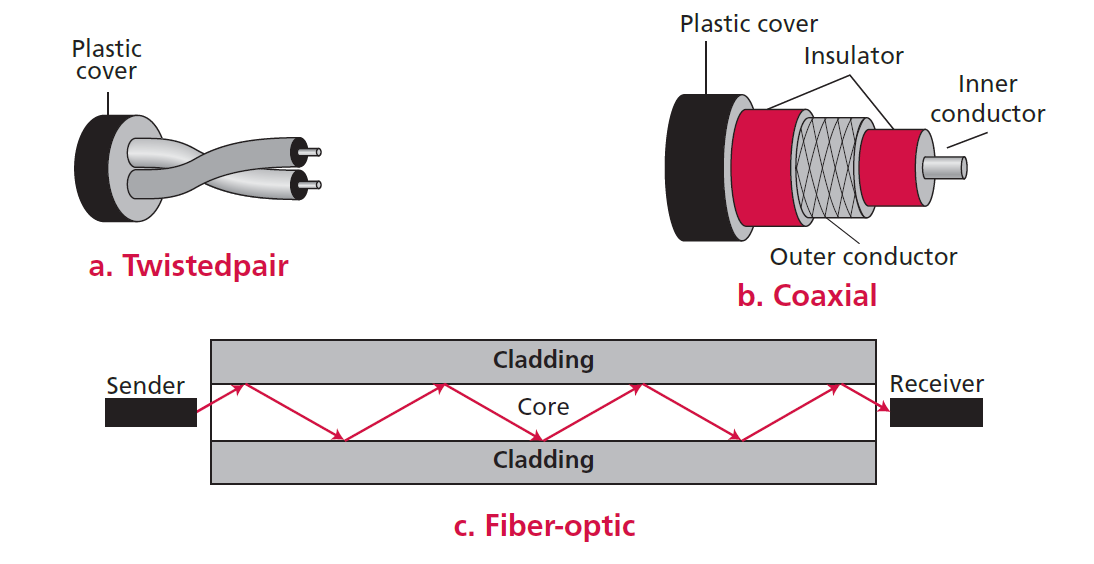
\includegraphics[width=0.6\textwidth]{\main/images/unit06/guided_media.png}
					\end{center}
				\end{definition}
				\begin{description}
					\item[Twisted-Pair Cable] Two conductors (normally copper), with plastic insulation, are twisted together. One wire carries signals to the receiver. The other is used as a ground reference.

						Interference may affect both wires. By twisting the cables, a balance is maintained between the data and the interference.

						DSL lines that are used by telephone companies use these cables.
					\item[Coaxial Cable] Instead of two wires, a central core conductor of solide or stranded wire (usually copper) is enclosed in an insulating sheath. This isa then encased in an outer conductor of metal foil, braid, or a combination of the two. The outer metallic wrapping works as a shield against noise, and as a second conductor. This outer conductor is enclosed in an insulating sheath, and the shole cable is protected by a plastic cover.

						Used by cable TV networks, although some TV providers have replaced this with fibre-optic cable.
					\item[Fibre-optic Cable] Made of glass or plastic, and transmits signals in the form of light. Uses the property of a mean of light that is refracted when it encounters a medium of less density. Covering a glass or plastic medium by another less dense medium (called \concept{cladding}) guides the light through the medium.

						Often found in backbone networks, as its wide bandwidth is cost-effective.
				\end{description}
			\subsection{Unguided Media}
				\begin{definition}{Wireless Communication}
					Transports electromagnetic waves without using a physical conductor. Uses three different ranges of electromagnetic spectrum: radio waves, microwaves, and infrared.
					\begin{center}
						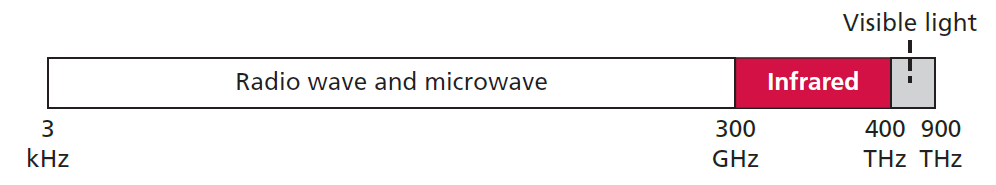
\includegraphics[width=0.7\textwidth]{\main/images/unit06/spectrum.png}
					\end{center}
				\end{definition}
				\begin{description}
					\item[Radio Waves] Frequencies between $3$ kHz and $1$ GHz. Mostly used for radio communication.
					\item[Microwaves] Frequencies between $1$ GHz and $300$ GHz. These are \concept{unidirectional} -- they can be narrowly focused. The sending and receiving antennas need to be aligned. This means that they do not interfere with another pair of aligned antennas.
					\item[Infrared] Frequencies from $300$ GHz to $400$ THz. Wavelengths from $1$ mm to $770$ nm. Used for short-range communication. Cannot penetrate walls. This therefore prevents interference between systems. However, this makes it useless for long-range communication. Cannot be used outside a building, as the sun's rays would interfere.
				\end{description}
	\rulechapterend
\end{document}